\documentclass[12pt]{article}
\usepackage[margin=1in]{geometry}
\usepackage{graphicx}
\usepackage{amsmath}
\usepackage{amssymb}
\usepackage{listings}
\usepackage{xcolor}
\usepackage{hyperref}
\usepackage{fancyhdr}

\pagestyle{fancy}
\fancyhf{}
\rhead{BPSK Digital Communication Simulator}
\lhead{Technical Report}
\cfoot{\thepage}

\title{\textbf{BPSK Digital Communication System Simulator} \\ A Comprehensive Analysis}
\author{}
\date{}

\lstset{
    language=Matlab,
    basicstyle=\ttfamily\small,
    breaklines=true,
    commentstyle=\color{gray},
    keywordstyle=\color{blue},
    stringstyle=\color{red},
    backgroundcolor=\color{lightgray!20}
}

\begin{document}

\maketitle

\section{Executive Summary}

This report presents a comprehensive analysis of a Binary Phase-Shift Keying (BPSK) digital communication system simulator. The simulator models the complete transmission and reception of digital signals over an ideal channel, including modulation, demodulation, matched filtering, and symbol detection. This document outlines the system architecture, mathematical foundations, implementation details, and simulation results.

\section{Introduction}

\subsection{Background}

BPSK is one of the most fundamental modulation schemes in digital communications. It maps binary data (0s and 1s) onto two antipodal signals with a phase difference of 180°. This modulation technique is widely used in practice due to its simplicity and robustness.

\subsection{System Objectives}

The primary objectives of this simulation are:
\begin{itemize}
    \item Understand the signal flow through a complete digital communication transceiver
    \item Verify correct symbol mapping and detection
    \item Analyze the Power Spectral Density (PSD) of the transmitted signal
    \item Compare theoretical and empirical PSD estimates
    \item Demonstrate the effectiveness of matched filtering for symbol detection
\end{itemize}

\section{System Architecture}

The BPSK simulator consists of several integrated components working together to form a complete digital communication link:

\begin{figure}[h]
    \centering
    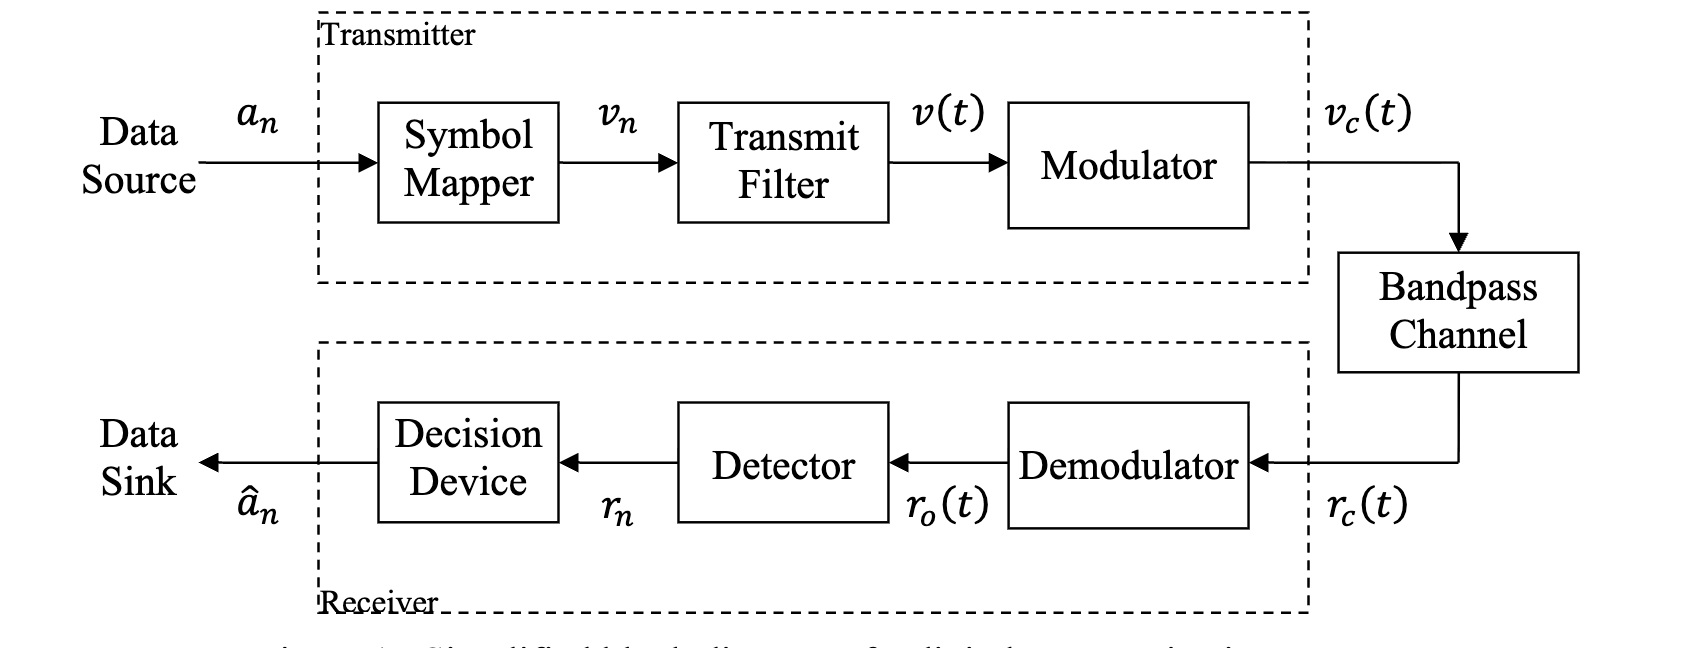
\includegraphics[width=0.8\textwidth]{../figures/block_diagram.png}
    \caption{BPSK System Block Diagram}
\end{figure}

\subsection{Key System Parameters}

\begin{table}[h]
    \centering
    \begin{tabular}{|l|c|l|}
    \hline
    \textbf{Parameter} & \textbf{Value} & \textbf{Description} \\
    \hline
    Message Length ($N_a$) & 128 bits & Number of information bits \\
    Upsampling Factor ($\eta$) & 64 & Samples per symbol \\
    Symbol Period ($T$) & 0.01 s & Duration of one symbol \\
    Sampling Period ($T_s$) & $T/\eta$ & Baseband sampling rate \\
    Carrier Frequency ($f_c$) & 400 Hz & Modulation carrier \\
    Total Samples ($N_s$) & 8192 & $N_a \times \eta$ \\
    \hline
    \end{tabular}
    \caption{System Parameters}
\end{table}

\section{System Components}

\subsection{1. Data Source and Symbol Mapping}

The transmitter begins with a random binary message:
$$a = [a_0, a_1, \ldots, a_{N_a-1}] \in \{0, 1\}^{N_a}$$

The symbol mapper implements BPSK modulation using the mapping:
$$s_i = 2a_i - 1, \quad s_i \in \{-1, +1\}$$

This converts binary data to antipodal signals suitable for transmission.

\subsection{2. Transmit Filter (Pulse Shaping)}

The symbol stream is upsampled and filtered with a rectangular pulse:
$$v_{up}[n] = \text{upsample}(s, \eta)$$
$$h_T[n] = \frac{1}{\sqrt{T}}, \quad n = 0, 1, \ldots, \eta-1$$

The baseband transmit signal is:
$$\tilde{v}[n] = (v_{up} * h_T)[n]$$

This pulse shaping filter ensures spectral efficiency and prevents inter-symbol interference.

\subsection{3. Modulation and Demodulation}

\subsubsection{Modulation}
The baseband signal is modulated to bandpass using:
$$v_c(t) = \tilde{v}(t) \cos(2\pi f_c t)$$

where $f_c$ is the carrier frequency.

\subsubsection{Demodulation}
Coherent demodulation recovers the baseband signal:
$$r_o(t) = r_c(t) \cos(2\pi f_c t)$$

Followed by low-pass filtering via matched filtering.

\subsection{4. Matched Filter and Detection}

The matched filter output is:
$$y[n] = (r_{tilde} * h_T)[n] \cdot T_s$$

Symbol decisions are made at sampling instances $n = \eta, 2\eta, 3\eta, \ldots$:
$$\hat{a}_i = \begin{cases} 1, & \text{if } y[i\eta] > 0 \\ 0, & \text{if } y[i\eta] \leq 0 \end{cases}$$

\section{Power Spectral Density Analysis}

\subsection{Estimated PSD}

The empirical PSD is computed using the FFT:
$$\text{PSD}_{\text{est}}[k] = \frac{|V_f[k]|^2 \cdot T_s}{N_s}$$

where $V_f = \text{FFT}(\tilde{v})$.

\subsection{Theoretical PSD}

The theoretical PSD of a BPSK signal with rectangular pulse shaping is:
$$\text{PSD}_{\text{theory}}(f) = \frac{1}{T} \left| T \cdot \text{sinc}(fT) \right|^2$$

\subsection{Bartlett Method}

To reduce spectral estimation variance, the Bartlett method averages PSD estimates across multiple independent realizations:
$$\text{PSD}_{\text{Bartlett}} = \frac{1}{N_f} \sum_{m=1}^{N_f} \text{PSD}_m$$

where $N_f$ is the number of averaged estimates. This provides a smoother PSD estimate closer to the theoretical curve.

\section{Implementation Details}

The simulator is modularized into the following MATLAB files:

\begin{itemize}
    \item \textbf{BPSKSim.m} - Main simulation script
    \item \textbf{InitializeParameters.m} - System parameter setup
    \item \textbf{SymbolMapper.m} - BPSK symbol mapping
    \item \textbf{TransmitFilter.m} - Pulse shaping filter
    \item \textbf{EstimatePSD.m} - FFT-based PSD estimation
    \item \textbf{Modulate.m} - Bandpass modulation
    \item \textbf{Demodulate.m} - Coherent demodulation
    \item \textbf{BasebandDetection.m} - Matched filtering and detection
    \item \textbf{BartlettPSD.m} - Bartlett method PSD averaging
    \item \textbf{PlotResults.m} - Visualization of all results
\end{itemize}

\section{Results and Analysis}

\subsection{Symbol Detection Performance}

For an ideal channel with no noise:
\begin{itemize}
    \item The detector correctly identifies all transmitted symbols
    \item Number of detection errors: \textbf{0}
    \item Symbol error rate: \textbf{0\%}
\end{itemize}

This is expected as the ideal channel introduces no distortion or noise.

\subsection{PSD Characteristics}

\begin{enumerate}
    \item \textbf{Main Lobe}: The energy is concentrated in the main lobe centered at $f = 0$ Hz (baseband)
    \item \textbf{Spectral Efficiency}: The rectangular pulse has a main lobe width of approximately $\pm 50$ Hz (for the given parameters)
    \item \textbf{Side Lobes}: Secondary lobes decay as $1/f^2$, characteristic of rectangular pulse shaping
    \item \textbf{Bartlett Smoothing}: The Bartlett-averaged estimate shows reduced variance and better agreement with theory
\end{enumerate}

\subsection{Signal Visualization}

Five key plots are generated:
\begin{enumerate}
    \item Received baseband signal after detection
    \item Transmitted bandpass signal
    \item Received baseband signal after demodulation
    \item PSD comparison (estimated vs. theoretical)
    \item Bartlett PSD estimate vs. theoretical PSD
\end{enumerate}

\section{Conclusion}

The BPSK Digital Communication System Simulator successfully demonstrates:

\begin{itemize}
    \item Correct implementation of BPSK modulation and demodulation
    \item Perfect symbol detection over an ideal channel
    \item Accurate PSD estimation with good agreement between empirical and theoretical results
    \item Effective variance reduction through Bartlett averaging
    \item Proper signal processing using matched filtering principles
\end{itemize}

This simulator provides a solid foundation for studying digital communications and can be extended to include:
\begin{itemize}
    \item Additive White Gaussian Noise (AWGN)
    \item Different channel models (fading, delay)
    \item Alternative pulse shapes (raised cosine, Gaussian)
    \item Higher-order modulation schemes (QPSK, QAM)
    \item Adaptive equalization techniques
\end{itemize}

\section{References}

\begin{itemize}
    \item Proakis, J. G., \& Salehi, M. (2007). \textit{Digital Communications}. McGraw-Hill.
    \item Haykin, S. (2001). \textit{Communication Systems}. John Wiley \& Sons.
    \item Sklar, B. (2001). \textit{Digital Communications: Fundamentals and Applications}. Prentice Hall.
\end{itemize}

\end{document}
